\documentclass[Visionprosjekt.tex]{subfiles} 
\NormalTopp
\begin{document} 

%%%%%%%%%%%%%%%%%%%%%%%%%%%%%%%%%%%%%%%%%%%%%%%%
\section{Elektriske komponenter}
%%%%%%%%%%%%%%%%%%%%%%%%%%%%%%%%%%%%%%%%%%%%%%%%

Dette kapitlet vil gi en  beskrivelse av de elektriske og elektroniske hovedkomponentene i prosjektet, og hvordan de er konfigurert.
I \reft{tab:elliste} er de viktigste elektroniske komponentene listet opp med referanse til koplingsskjemaene og blokkdiagrammene. Koplingsskjemaer med tilhørende  koplingstabeller finnes i \refv{ved:skjema}.
De neste underkapitlene vil beskrive de elektriske enhetene nærmere.

%
%\begin{table}[ht]%
    %\centering
    %\caption{Materialliste}
    %\renewcommand\arraystretch{1.5}
    %\begin{tabularx}{\textwidth}{c>{\raggedright}p{40mm}X}
        %\toprule
        %Ant.	& Typebetegnelse			&  Beskrivelse\\
        %\midrule
        %1		& Peli Storm Case iM2600	&  Koffert som fungerer som kapsling for alle enheter.\\
        %\bottomrule
	%\end{tabularx}
    %\label{tab:materialliste}
%\end{table}




\begin{table}[ht]%
    \centering
    \caption{Elektriske hovedkomponenter}    
    \renewcommand\arraystretch{1.2}
    %\small %
    \footnotesize
    \begin{tabularx}{\textwidth}{cll>{\raggedright\arraybackslash}p{22mm}>{\raggedright\arraybackslash}X}
        \toprule
        Ant. & Produsent	& Modell  & Referanse & Beskrivelse\\
        \midrule
        1 &  Pepperl+Fuchs  & SB4   & SB      & Sikkerhetsmonitor.\\
        1 & Siemens & S7-300        & PLS     &  Siemens Simatic S7 PLS, ikke montert på brettet.\\
        1 & Siemens & ET 200M       & PLS0, PLS2, PLS4         & Ekstern digital I/O-modul for PLS. Med Profibus DP-tilkopling.\\
        6 &   SICK  & WT 42P330     & FCM1--FCM4, \newline FC1, FC3 &  Brukt ved start, til muting og ved fyllestasjon. 
        Optisk sensor  med rekkevidde inntil 13\,cm.\\
        1 & Fotek   &  DR-30X       & FC2  	& Optisk sensor ved vision-kamera.\\
        1 & Mean Well & Q-120D      & PSU1    & Strømforsyning, 12 og 24\,V. \\
        1 & Cognex  & DVT530      & CAM     & Vision-kamera.\\
        1 & Cognex  & DVT BOB     & DVT     & I/O-modul for vision-kamera.\\
        1 &  ABB    & ACS355      & VFD1    & Frekvensomformer.\\
        1 &  ABB    & FPBA-01     &         & Profibus-adapter for frekvensomformeren.\\
        1 & Parker Lucifer & 341P01   & MV1  	& Elektrisk 5/2-pneumatikkventil.\\
        2 & Micro motors & TH158.24.510& M2, M3 	& Matemotorer.\\
        3 & Repol   & R4-214-23-1024-WT   & K1--K3 	& Releer.\\
        2 & Aeco    & INZAGO        & LZ1--LZ2	& Nivåsensorer.\\
        2 &  Pepperl+Fuchs          & CBB4-12GH70-E2   & LZ3--LZ4	& Impellersensorer.\\
        1 & Merlin Gerin & C60H     & F1	& Jordfeilautomat \\
        \bottomrule
	\end{tabularx}
    \label{tab:elliste}
\end{table}













%
%%%%%%%%%%%%%%%%%%%%%%%%%%%%%%%%%%%%%%
%\subsection{PLS-system}
%%%%%%%%%%%%%%%%%%%%%%%%%%%%%%%%%%%%%%
%
%PLS-systemet består av følgende
%
%\begin{itemize}
	%\item Strømforsyning \red{PS\_PLS}
    %\item Siemens S7 PLS
    %\item Ekstern digital IO-modul
%\end{itemize}


\clearpage
%%%%%%%%%%%%%%%%%%%%%%%%%%%%%%%%
\subsection{Sikkerhetsmonitor}
%%%%%%%%%%%%%%%%%%%%%%%%%%%%%%%%


%\begin{figure}[ht]

\begin{wrapfigure}{r}{55mm}
	\centering
    \vspace{-10pt}
		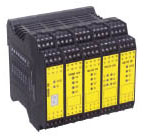
\includegraphics{bilder/sb4.jpg}
	\caption{SafeBox SB4}
	\label{fig:sb4}
\end{wrapfigure}


Dette underkapitlet er basert på manualen til SafeBox \cite{sb4}. For å ivareta sikkerheten rundt sorteringsanlegget, er sikker\-hets\-monitoren «SafeBox SB4» benyttet, vist på \reff{fig:sb4} \cite{sb4bilde}. Hensikten med denne er å stanse bevegelige deler dersom en   farlig situasjon oppstår. %Hvis nødstoppbryteren blir aktivert vil også matemotorene stoppe, og luftstempelet vil trekke seg tilbake. 
En farlig situasjon detekteres vha. en sikkerhetsstråle satt opp på tvers av båndet, før plasttunnelen. Sensorer som midlertidig deaktiverer sikkerhetsstrålen, kalt «mutingsensorer», gjør det mulig å sende inn beholdere som bryter strålen uten at anlegget stoppes. Mutingsensorene er en del av sikkerhetsystemet, og er derfor tilkoblet sikkerhetsmonitoren. 

%\begin{figure}[ht]
	%\centering
		%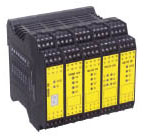
\includegraphics{bilder/sb4.jpg}
	%\caption{SafeBox SB4}
	%\label{fig:sb4}
%\end{figure}



SafeBox SB4 er en konfigurerbar sikkerhetsmonitor fra Pepperl+Fuchs. Den består av et kabinett hvor det kan installeres inntil seks forskjellige sikkerhetsmoduler for å oppnå ønsket funksjon. I \reft{tab:sbmoduler} er  alle modulene som er benyttet i SafeBox-kabinettet beskrevet, samt deres plassering. De to første modulene (montert til venstre) er påkrevd for å få en fungerende sikkerhetsmonitor. 



\begin{table}[ht]
\centering
    \caption{Moduler som er brukt i SafeBox SB4.}
    \renewcommand\arraystretch{1.2}
    \small
    \begin{tabularx}{\textwidth}{clX}        
        \toprule
        Plass	&	SB4 Modul &	Beskrivelse																			\\
        \midrule
        1		&	OR	  &	Strømforsyning, reléutganger og innganger for nullstilling. Denne modulen er obligatorisk.						\\
        2		&	4CP	  &	Mikrokontroller for hele kabinettet, samt fire innganger for sikkerhetssensorer. 
        Denne modulen er obligatorisk.						\\
        3		&	4M	  &	«Mutingmodul» med opptil fire mutingsensorer. Deaktiverer («muter») modulen til venstre i kabinettet.			\\
        4		&	2E	  &	Nødstoppmodul med to innganger og to reléutganger. 							\\
        5		&   4C	  &	Modul som ligner på 4CP, men er uten mikrokontroller. Har fire sensorinnganger.	Denne er ikke i bruk i anlegget.\\
       \bottomrule
    \end{tabularx}
    \label{tab:sbmoduler}
\end{table}



Sikkerhetsmonitoren er konfigurert i henhold  til tidsdiagrammene vist på \reff{fig:seqTiming}. Høyt nivå på «Sikkerhetsstråle» indikerer at denne er brutt.
Mutingsensorene detekterer beholderne sekvensielt, slik at FCM1 og FCM3 blir aktivert samtidig, før FCM1 faller ut. Plasseringen av sensorene er vist på anleggstegningen, \reff{fig:systemfigur2}.


Alle modulene som er montert i sikkerhetsmonitoren er utstyrt med DIP-brytere for å kunne tilpasse deres funksjon. De neste underkapitlene vil gi en detaljert beskrivelse av modulene, og hvordan  DIP-bryterne er innstilt.


%\begin{figure}[ht]
	%\centering
    %%
\includegraphics[scale=2]{logobilder/pi.jpg}
    %\begin{tikztimingtable}[
    %timing/slope=0,         % no slope
    %timing/coldist=2pt,     % column distance
    %xscale=2.8,yscale=1.4,      % scale diagrams
    %thick ,              % set line width
    %timing/font=\normalfont
    %]
          %FCM1    & 16{C}  0.5C\\
          %FCM2    & 8{2C}  0.5C\\
          %FCM3    & 4{4C}  0.5C\\
          %FCM4    & 2{8C}  0.5C\\
        %\\
        %Muting & HLLHHHHXXLLHHXL\\
        %\extracode 
        %\begin{pgfonlayer}{background}
            %\begin{scope}[gray,semitransparent,semithick]
                %%\horlines{}
                %\vertlines{}
            %\end{scope}
            %\node[anchor=north west, inner sep=0pt] at (5,-7) {\footnotesize $\leftarrow$ positive edge triggered $\rightarrow$};
        %\end{pgfonlayer}
    %\end{tikztimingtable}
    %%\put(-200,0){\fcolorbox{white}{white}{Boks inne}}
    %%\put(-300,30){\fcolorbox{white}{white}{$\xleftarrow{\hspace*{2cm}}$ Boks inne $ \xrightarrow{\hspace*{2cm}}$}}
    %\caption{Timingdiagram -- fullstendig}
    %\label{fig:timingFull}
%\end{figure}

%  \makebox[width][position]{text}
\begin{figure}[ht]
	\centering
   % 
\includegraphics[scale=1]{logobilder/pi.jpg}
    \begin{tikztimingtable}[
    timing/slope=0,         % no slope
    timing/coldist=2pt,     % column distance
    xscale=3.3,yscale=1.4,      % scale diagrams
    thick ,              % set line width
    timing/font=\normalfont\small
    ]
          FCM1    & LHHHHHHHLLLLL 0.5L        \\
          FCM2    & LLHHHHHHHHLLL 0.5L        \\
          FCM3    & LLLLLLLHHHHHL 0.5L        \\
          FCM4    & LLLLLLLLLHHHH 0.5L        \\
        \\
        \parbox[c]{25mm}{\flushright Sikkerhets\-stråle}& LLLHHHHHHHHLL 0.5L       \\
        \\
        Muting   & LLHHHHHHHHHHL 0.5L          \\
        \extracode
        \begin{pgfonlayer}{background}
            \begin{scope}[gray,semitransparent,semithick]
                \horlines{}
                %\draw (0,0) node[] {The quick brown fox jumps over the lazy dog.};
                \vertlines{}
            \end{scope}
            %\node[anchor=north west, inner sep=0pt, text width=2cm] at (-2,0) {\footnotesize Sikkerehetssensor};
        \end{pgfonlayer}
    \end{tikztimingtable}
    \caption{Tidsdiagram -- typisk}
    \label{fig:seqTiming}
\end{figure}




\newlength{\kolbreddeA}
\settowidth{\kolbreddeA}{DIP4:}

\newlength{\kolbreddeB}
\settowidth{\kolbreddeB}{OFF,}

\newcolumntype{d}{p{\kolbreddeA}}
\newcolumntype{s}{p{\kolbreddeB}}




\subsubsection{SB4 Modul OR}
SB4 Modul OR består av strømforsyning for hele sikkerhetsmonitoren, og må plasseres helt til venstre i kabinettet. Modulen har  innganger for overvåking av sikkerhetsrelé, gjenstart (restart), nullstilling (reset) og to potensialfrie kontakter som kobler ut dersom sikkerhetsmonitoren går i sikkermodus. Konfigureringen
\begin{center}
    \begin{tabular}{dssss}  
        DIP1: & OFF&OFF&OFF&OFF
    \end{tabular}
\end{center}
deaktiverer automatisk gjenstart og sikkerhetsrelé-overvåking.





\subsubsection{SB4 Modul 4CP}
SB4 Modul 4CP inneholder en mikrokontroller som er felles for hele kabinettet, og må plasseres til høyre for SB4 Modul OR. Modulen har i tillegg fire innganger hvor brytere eller lysgardiner kan kobles til. Sikkerhetssensorene FCT1 og FCR1 er tilkoblet her. Det er disse som setter opp sikkerhetsstrålen. Med konfigurasjonen 
\begin{center}
    \begin{tabular}{dssss}  
        DIP1: & OFF&OFF&OFF&OFF
    \end{tabular}
\end{center}
vil modulen ha og-funksjon mellom inngangene. I sorteringsanlegget er det brukt én sikkerhetsstråle, de tre andre inngangene er lasket til logisk 1. Dermed vil sikkerhetsstrålen styre statusen direkte.








\subsubsection{SB4 Modul 4M}
SB4 Modul 4M er en mutingmodul som vil deaktivere inngangene i modulen den står til høyre for. Denne modulen har fire innganger hvor mutingsensorene FCM1, FCM2, FCM3 og FCM4 er tilkoblet. Konfigurasjonen
\begin{center}
    \begin{tabular}{dssss}  
        DIP1: & ON&OFF&OFF&OFF\\
        DIP2: & ON&OFF&OFF&OFF
    \end{tabular}
\end{center}
gir sikkerhetsmonitoren følgende funksjoner:
\begin{itemize}
	\item Overvåking av muting-lampe er aktivert.
    \item Maksimaltid for mutingsensorer å ligge inne er 4\,minutter.
    \item  Enkel muting er aktivert, dvs. en sensor på hver side av lysgardinen (FCM2 og FCM3) kan holde mutingen. Se tidsgdiagram i \reff{fig:seqTiming}.
\end{itemize}




\subsubsection{SB4 Modul 2E}
Grupperingsmodulen SB4 Modul 2E  kan settes til stoppkategori 0 eller 1 med tidsforsinkelse. Den har to potensialfrie kontakter som kobler ut hvis en modul i gruppa går i sikkerhetsmodus (dersom DIP-bryterne velges slik at kategori 1 oppnås, vil også SB4 Modul OR gå i sikkerhetsmodus). DIP-bryterne er satt til 
\begin{center}
    \begin{tabular}{dssss}  
        DIP1: & OFF&OFF&OFF&OFF\\
        DIP2: & OFF&OFF&OFF&OFF\\
        DIP3: & ON&OFF&OFF&OFF\\
        DIP4: & ON&OFF&OFF&OFF,
    \end{tabular}
\end{center}
som betyr at tidsforsinkelsen ved stoppkategori 1-operasjon er 0 s, at modulen er satt til stoppkategori 0, og sikkerhetsrelé-overvåking og gjenstart er avslått.







\subsubsection{SB4 Modul 4C}
SB4 Modul 4C er ikke i bruk,  inngangene er lasket for å hindre utløsning av sikkerhetsmodus.
Denne modulen har fire innganger som det kan kobles på opptil fire lysgardiner eller brytere. DIP-bryterne er satt til 
\begin{center}
    \begin{tabular}{dssss}  
        DIP1: & OFF&OFF&OFF&OFF,
    \end{tabular}
\end{center}
som betyr at eksklusiv eller-funksjon og simultan overvåking på to og to av inngangene er avslått. Modulen har samme virkemåte som SB4 Modul 4CP, men mangler mikrokontroller. Siden modulen i dette tilfellet er plassert etter SB4 Modul 2E, vil den tilhøre SB4 Modul 2E sin gruppe. Det vil si at denne modulen kun vil trigge SB4 Modul 2E over i sikkerhetsmodus, mens SB4 Modul OR vil kjøre normalt.




%%%%%%%%%%%%%%%%%%%%%%%%%%%%%%%%
\subsection{Frekvensomformer}
%%%%%%%%%%%%%%%%%%%%%%%%%%%%%%%%

Frekvensomformeren ABB ACS355 er benyttet i prosjektet til å styre hastigheten til båndet, samt å generere trefaset spenning.  Frekvensomformeren er vist på \reff{fig:frekvensomformer}. For å muliggjøre kommunikasjon over Profibus DP, er frekvensomformeren utstyrt med adapteren ABB PROFIBUS DP Adapter Module FPBA-01. 

I \reft{tab:frekvens} er nøkkeldata for frekvensomformeren listet opp.


\begin{figure}[ht]
    \begin{minipage}[c]{0.65\textwidth}
      %  \begin{table}[ht]
        \centering
            \caption{Nøkkeldata for ABB ACS355 \cite{frekvensdata}}
            \renewcommand\arraystretch{1.2}
            \begin{tabular}{llX}        
                \toprule
                Egenskap	&	Verdi					 \\
                \midrule
                Typebetegnelse        & ACS355-01E-02A4-2\\
                Innspenningsområde    & 200--240\,VAC    \\
                Frekvensområde ut     & 0--600\,Hz       \\
                Maksimal belasting    & 370\,W, 2,4\,A   \\
               \bottomrule
            \end{tabular}
            \label{tab:frekvens}
        %\end{table}
    \end{minipage}
    %\hspace{0.2cm}
    \begin{minipage}[c]{0.25\textwidth}
        \centering
        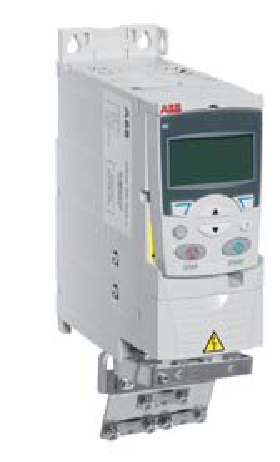
\includegraphics[height=4cm]{bilder/frekvensomformer.pdf}
        \caption{\mbox{Frekvens}\-\mbox{omformeren}}
        \label{fig:frekvensomformer}
    \end{minipage}
\end{figure}

%
%\begin{table}[ht]
%\centering
    %\caption{Nøkkeldata for ABB ACS355 \cite{frekvensdata}.}
    %\renewcommand\arraystretch{1.2}
    %\begin{tabular}{llX}        
        %\toprule
        %Egenskap	&	Verdi					 \\
        %\midrule
        %Typebetegnelse        & ACS355-01E-02A4-2\\
        %Innspenningsområde    & 200--240\,VAC    \\
        %Frekvensområde ut     & 0--600\,Hz       \\
        %Maksimal belasting    & 370\,W, 2,4\,A   \\
       %\bottomrule
    %\end{tabular}
    %\label{tab:frekvens}
%\end{table}
%




%\clearpage
\subsubsection{Konfigurering}

Nødstoppsignalet fra sikkerhetsmonitoren er tilkoblet digitalinngangen DI1 i frekvensomformeren for å gjøre nødstoppfunksjonen uavhengig av bussystemet. 
For å kunne stoppe frekvensomformeren  med DI1, må dette settes opp i konfigurasjonen. 


Det elektroniske motorvernet må stilles inn på nominell belastningsstrøm, som her er $I_B = 0,4$\,A.
\refT{tab:frekvensparametre} gir en oversikt over innstillinger som er forandret i frekvensomformeren.

\begin{table}[ht]%
    \centering
    \caption{Innstillinger for frekvensomformer.}
    \label{tab:frekvensparametre}
        \renewcommand\arraystretch{1.2}
    \begin{tabularx}{0.85\textwidth}{>{\ttfamily}l>{\ttfamily}l>{\raggedright\arraybackslash}X}
    \toprule
        \normalfont Parameter	& \normalfont Verdi		&	Beskrivelse\\
    \midrule
		2003 MAX CURRENT		&	0.4 A		&	Definerer høyeste motorstrøm \\
		2021 MAX SPEED SEL		&	EXT REF 1	&	Høyeste hastighet er valgt av høyeste referansefrekvens \\
		2109 EMERG STOP SEL		&	DI1 (INV)	&	Nødstoppsignal tilkobles DI1 \\
        \bottomrule
    \end{tabularx}
\end{table}




%%%%%%%%%%%%%%%%%%%%%%%%%%%%%%%%
\subsection{Sensorer}
%%%%%%%%%%%%%%%%%%%%%%%%%%%%%%%%


For å detektere posisjonen til beholderen på transportbåndet og muting av sikkerhetsstrålen, er det brukt optiske og  kapasitive sensorer. %Signaler fra sensorene brukes til aktivering av oppgaver eller muting av sikkerhetssystemer. 
Nedenfor er sensortypene og bruksområdene beskrevet. 


\begin{description}[style=multiline,leftmargin=24mm]
	\item[Optiske sensorer] 
            Ved fyllestasjonen, sikkerhetsmonitoren og materampen er det montert optiske sensorer av typen SICK WT 4-2. Sensorene sender ut rødt lys og detekterer om dette blir reflektert av et objekt, innenfor en avstand på maksimalt 13\,cm. Sensorene har høy immunitet mot fremmedlys. De krever 10--30\,VDC drivspenning.
	\item[Kapasitive sensorer] 
            Kapasitive sensorer brukes for nivådetektering i pelletsbeholderne, bulktellere ved mateskruene og for kamera-aktivering. Sensortypen detekterer endringer i dielektrikumet (isolasjonsmaterialet mellom elektrodene i en kondensator) i måleområdet. 
 Sensorene trenger en drivspenning på 5--28\,VDC. 
\end{description}

Alle sensorer benyttet i dette prosjektet gir binære verdier -- aktivert eller ikke aktivert.





%%%%%%%%%%%%%%%%%%%%%%%%%%%%%%%%
\subsection{Pneumatikk}
%%%%%%%%%%%%%%%%%%%%%%%%%%%%%%%%

Sylinderen som skyver beholderne av transportbåndet er pneumatisk styrt. Det benyttes en dobbeltvirkende sylinder med endeposisjon inne og ute. Sensorene LZ5 (ute) og LZ6 (inne) detekterer om stempelet er i en av endeposisjonene.

For å styre  lufttilførselen til sylinderen brukes en magnetisk styrt 5/2-ventil\footnote{«5/2» vil si at ventilen har 5  tilkoplinger og  2 stabile posisjoner.} %Bruk av 5/2-ventiler er vanlig i pneumatikksystemer med dobbeltvirkende sylindere.}. 
Sylinderen er koplet opp som vist i \reff{fig:luftvent}, her er trykkluf ført inn på tilkopling 1.

\begin{figure}[ht]
\centering
		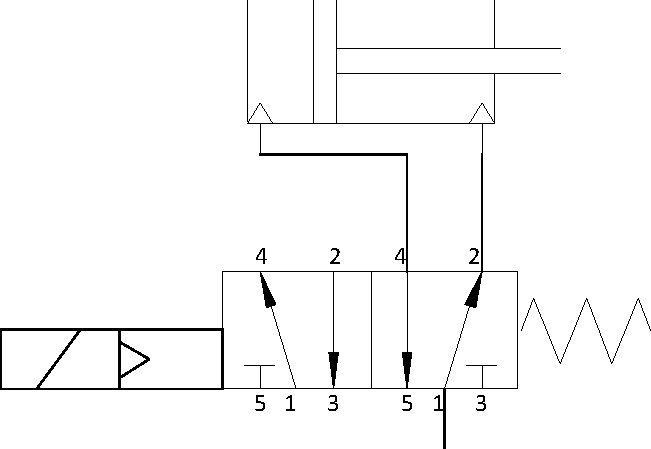
\includegraphics[scale=0.7]{bilder/luftstyring.pdf}
	\caption{Pneumatikksylinder med styreventil}
	\label{fig:luftvent}
\end{figure}







\newpage
Nedenfor er virkemåten til det pneumatiske systemet forklart.
%Det pneumatiske systemet fungerer på følgende måte.
\begin{itemize}
	\item Når ventilen ikke er aktivert (spenningsløs), slippes trykkluft fra tilkobling 1 til 2 og inn på «høyresiden» av stempelet. Lufta på den andre siden av stempelet slippes gjennom 4--5 og ut i friluft. Stempelet vil dermed bli hold inne. \refF{fig:luftvent} viser ventilen i denne posisjonen.
  \item  Ved aktivering av ventilen slippes trykkluft inn på «venstresiden» av stempelet via tilkopling 1 og 4. Via 2--3 slippes lufta fra den andre siden  ut i friluft. Stempelet vil med dette presses ut. 
\end{itemize}

Sylinderen har reduksjonsventiler på luftinnløpene. Reduksjonsventilene er brukt til å strupe luftstrømmen for å redusere hastigheten på stempelet ved inn- og utskyvning. Dette hindrer potensielt farlige situasjoner og øker presisjonen til skyvearmen.







\end{document}

